\subsection{Overview}
\begin{frame}
	\frametitle\insertsection
	\framesubtitle\empty
	\begin{center}
		\Large \textbf{\insertsubsection}
	\end{center}
\end{frame}
\begin{frame}
	\frametitle\insertsection
	\framesubtitle\insertsubsection
	\vspace{-2em}
	\begin{block}{Association}
		Process of assigning measurements to existing tracks or existing tracks to measurements (measurement-to-track association vs. track-to-measurement association).
	\end{block}
	\begin{itemize}
		\item {Correlations may be ambiguous.}
		\item {Association determines how the reports are used to update tracks.}
		\item {In general, there are more than $N$ measurements and $M$ tracks possible for association.}
		\item {Needs a metric and a decision criteria to resolve ambiguities.}
	\end{itemize}
\end{frame}
\begin{frame}
	\frametitle\insertsection
	\framesubtitle\insertsubsection
	\vspace{-2em}
	\begin{block}{Data Association Algorithms}
		\begin{itemize}
			\item {Global Nearest Neighbors Data Association (GNN-DA)}
			\item {Probabilistic Data Association (PDA)}
			\item {Joint Probabilistic Data Association (JPDA)}
			\item {Multi Hypothesis Testing (MHT)}
		\end{itemize}
	\end{block}
\end{frame}
\subsection{Global Nearest-Neighbors Data Association}
\begin{frame}
	\frametitle\insertsection
	\framesubtitle\empty
	\begin{center}
		\Large \textbf{\insertsubsection}
	\end{center}
\end{frame}
\begin{frame}
	\frametitle\insertsection
	\framesubtitle\insertsubsection
	\vspace{-2em}
	\begin{itemize}
		\item {An hard association.}
		\item {Considers tracks independently.}
		\item {Statistical distance of each measurement from track prediction is computed:}
		\begin{align*}
			D = (y_{k} - \hat{y}_{k|k-1})^{T}S^{-1}_{k|k-1}(y_{k}-\hat{y}_{k|k-1})
		\end{align*}
		\item {Select measurements validated inside the ellipsoidal gate for each track.}
		\item {Allow us building an assignment matrix.}
	\end{itemize}
\end{frame}
\begin{frame}
	\frametitle\insertsection
	\framesubtitle\insertsubsection
	\vspace{-2em}
	\begin{figure}
		\caption{\textbf{Example of data association conflict situation}}
		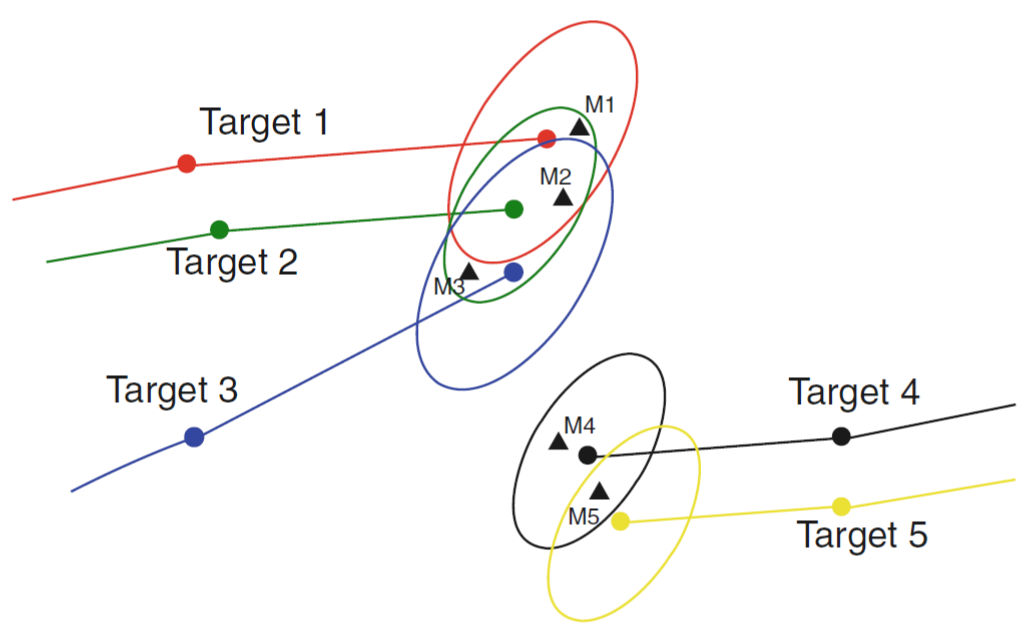
\includegraphics[scale=0.5]{./img/association}
	\end{figure}
\end{frame}
\begin{frame}
	\frametitle\insertsection
	\framesubtitle\insertsubsection
	\vspace{-2em}
	From this example, the assignment matrix can be given following:
	\begin{table}
		\begin{tabular}{| c | c | c | c | c | c |} \hline
			\rowcolor{aerolightblue}
			\textbf{} & \textbf{Target 1} & \textbf{Target 2} & \textbf{Target 3} & \textbf{Target 4} & \textbf{Target 5} \\ \hline
			\textbf{M1} & x & & & &\\ \hline
			\textbf{M2} & x & x & x & &\\ \hline
			\textbf{M3} & & x & x & &\\ \hline
			\textbf{M4} & & & & x &\\ \hline
			\textbf{M5} & & & & x & x\\ \hline
		\end{tabular}
	\end{table}
\end{frame}
\begin{frame}
	\frametitle\insertsection
	\framesubtitle\insertsubsection
	\vspace{-2em}
	\textbf{Optimal Assignment}
	\begin{itemize}
		\item {Gives the maximum number of possible assignment}
		\item {Minimizes the total squared distance for every track $i$ and measurement $j$.}
		\begin{align*}
		\min_{i,j} \sum_{i,j} D(i,j)
		\end{align*}
		\item {Finds the best overall global solution at the current time.}
	\end{itemize}
\end{frame}
\begin{frame}
	\frametitle\insertsection
	\framesubtitle\insertsubsection
	\vspace{-2em}
	\begin{table}
		\caption{\textbf{Assignment Matrix}}
		\begin{tabular}{| c | c | c | c | c | c |} \hline
			\rowcolor{aerolightblue}
			\textbf{} & \textbf{Target 1} & \textbf{Target 2} & \textbf{Target 3} & \textbf{Target 4} & \textbf{Target 5} \\ \hline
			M1 & \textbf{2} & $\infty$ & $\infty$ & $\infty$ & $\infty$ \\ \hline
			M2 & \textbf{7} & \textbf{3} & \textbf{4} & $\infty$ & $\infty$\\ \hline
			M3 & $\infty$ & \textbf{5} & \textbf{2} & $\infty$ & $\infty$\\ \hline
			M4 & $\infty$ & $\infty$ & $\infty$ & \textbf{2} & $\infty$\\ \hline
			M5 & $\infty$ & $\infty$ & $\infty$ & \textbf{3} & \textbf{2}\\ \hline
		\end{tabular}
	\end{table}
\end{frame}
\begin{frame}
	\frametitle\insertsection
	\framesubtitle\insertsubsection
	Determine the shortest distance from all possible solutions:
	\begin{table}
		\begin{tabular}{| c | c | c | c | c | c | c |} \hline
			\rowcolor{aerolightblue}
			\textbf{} & \textbf{Target 1} & \textbf{Target 2} & \textbf{Target 3} & \textbf{Target 4} & \textbf{Target 5} & $\sum D$ \\ \hline
			1 & M1,M2 & M3 &  & M4,M5 & & 19\\ \hline
			2 & M1,M2 & M3 &  & M4 & M5 & 18\\ \hline
			3 & M1,M2 & & M3 & M4,M5 & & 16 \\ \hline
			4 & M1,M2 & & M3 & M4 & M5 & 15 \\ \hline
			5 & M1 & M2 & M3 & M4,M5 & & 12 \\ \hline
			\rowcolor{green!50} 6 & M1 & M2 & M3 & M4 & M5 & 11 \\ \hline
			7 & M1 & M3 & M2 & M4,M5 & & 16 \\ \hline
			8 & M1 & M3 & M2 & M4 & M5 & 15 \\ \hline
			9 & M1 & M2,M3 & & M4,M5 & & 15 \\ \hline
			10 & M1 & & M2,M3 & M4 & M5 & 14 \\ \hline
		\end{tabular}
	\end{table}
\end{frame}
\begin{frame}
	\frametitle\insertsection
	\framesubtitle\insertsubsection
	\vspace{-2em}
	\begin{table}
		\caption{\textbf{Assignment Results}}
		\begin{tabular}{| c | c | c | c | c | c |} \hline
			\rowcolor{aerolightblue}
			\textbf{} & \textbf{Target 1} & \textbf{Target 2} & \textbf{Target 3} & \textbf{Target 4} & \textbf{Target 5} \\ \hline
			\textbf{M1} & \cellcolor{green!50}x & & & &\\ \hline
			\textbf{M2} & x & \cellcolor{green!50}x & x & &\\ \hline
			\textbf{M3} & & x & \cellcolor{green!50}x & &\\ \hline
			\textbf{M4} & & & & \cellcolor{green!50}x &\\ \hline
			\textbf{M5} & & & & x & \cellcolor{green!50}x\\ \hline
		\end{tabular}
	\end{table}
\end{frame}
\subsection{Assignment Algorithms}
\begin{frame}
	\frametitle\insertsection
	\framesubtitle\empty
	\begin{center}
		\Large \textbf{\insertsubsection}
	\end{center}
\end{frame}
\begin{frame}
	\frametitle\insertsection
	\framesubtitle\insertsubsection
	\vspace{-2em}
	\begin{itemize}
		\item {Hungarian or Munkres}
		\item {Auction}
		\item {Shortest Augmenting Path (JV--Jonker-Volgenant)}
		\item {JVC (Jonker-Volgenant-Castanon)}
		\begin{itemize}
			\item { A combination of the JV and Auction algorithms}
		\end{itemize}
		\item {These all give the same answer but differ in efficiency. }
	\end{itemize}
\end{frame}